 \item Usunięcie części - scenariusz główny \\
 
 Opis słowny - ten przypadek użycia opisuje funkcjonalność usuwania istniejących typów części. Obejmuje to sytuację, gdy np. sklep decyduje się na usunięcie starego asortymentu ze sprzedaży.
 
 \begin{longtable}{|p{5cm}|p{7cm}|}
 	\hline
	\textbf{Aktor} & Pracownik \\
	\hline
	\textbf{Warunki początkowe} & Posiadanie konta z uprawnieniami umożliwiającymi zarządzanie częściami, zalogowanie się do systemu \\
	\hline
	\textbf{Opis przebiegu interakcji} & Wybór prezentacji listy części na stronie głównej sklepu, wybranie opcji usunięcia konkretnej części, zatwierdzenie operacji \\
	\hline
	\textbf{Sytuacje wyjątkowe} & Istnieje niezerowa liczba części tego typu w magazynie \\
	\hline
	\textbf{Warunki końcowe} & Usunięcie z systemu wybranego typu części \\
	\hline
 \end{longtable}
 
  \item Usunięcie części - scenariusz główny \\
  \begin{tabularx}{\linewidth}{ c X}
  Aktor: & Pracownik \\
  \end{tabularx}
   \begin{enumerate}
    \item Scenariusz ``Wyświetlanie listy części - scenariusz alternatywny - użytkownik posiada specjalne uprawnienia do zarządzania częściami''. \label{usuniecie-czesci-poczatek}
    \item Pracownik wyszukuje na liście część którą chce usunąć i wybiera przycisk usunięcia. \label{usuniecie-czesci-wybor}
    \item System prosi użytkonika o potwierdzenie operacji.
    \item Pracownik zatwierdza operację.
    \item System usuwa część z bazy danych i informuje użytkownika o zakończeniu operacji.
  \end{enumerate}
  
  \item Dodanie części - scenariusz alternatywny - istnieje niezerowa liczba części tego typu w magazynie \\
  \begin{tabularx}{\linewidth}{ c X}
  Aktor: & Pracownik \\
  \end{tabularx}
   \begin{enumerate}
    \item Kroki \ref{usuniecie-czesci-poczatek} do \ref{usuniecie-czesci-wybor} scenariusza głównego.
    \item System sprawdza czy w magazynie znajdują się części danego typu. Jeśli tak (na magazynie znajduje się co najmniej 1 sztuka danego typu części), informuje o tym pracownika w formie ostrzeżenia.
    \item Powrót do scenariusza głównego.
  \end{enumerate}
  	
\begin{figure}[h!]
    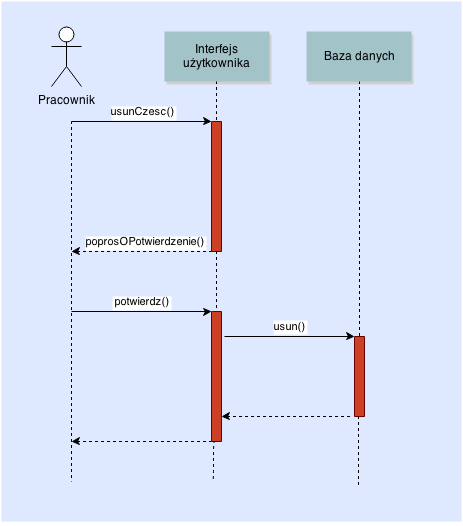
\includegraphics[width=\textwidth,
    height=0.7\textheight]{graphics/UseCase/Czesci/UsuniecieCzesciSD.png}
  \caption{Diagram sekwencji dla przypadku użycia Usunięcie części - scenariusz główny}
\end{figure}